\section{Morfeas WEB IOBOX-if/Portal UI}

The ``Morfeas WEB IOBOX-if/Portal" can be accessed from the Morfeas WEB front page by the button with the identical label.
An example of the ``Morfeas WEB IOBOX-if/Portal UI" derived at figure \ref{fig:IOBOX-if_UI}.
At the top left corner are a drop down menu that can select the IOBOX component under interest, by it's defined name.\\

\noindent The ``Morfeas WEB IOBOX-if/Portal UI" split in three sections.
The to drop down menu that explained above, the status box, and the measurement table.
The status text box show the last update (fetch) date, or the last error that happens.
The measurement table on the upper side show the configuration of the component together with the connection status.
The lower part contains that measurements that comes from the IOBOX.\\

\noindent The next section of the measurement table is the ``Wireless Inductive Power Supply" section.
This section provide the voltage and current measurements from the IOBOX's inductive power supply.
This Power supply have 4 outputs that controlled by some buttons on the IOBOX's front panel.\\

\noindent The followed four section provide the measurement of the telemetries.
The upper row of each telemetry measurements section, show the order name and the state of the receiver followed from the reception success rate indicator (RSSID).
The next lines have the measurements of each acquisition channel of the telemetry.
In case that the telemetry is out of power/range or the RF Channels is not configured the section filled with the word: \textbf{Disconnected}.\\

\noindent The RF channels can be configured only (unfortunately) by a proprietary software that given by the manufacture.

\begin{figure}[h]
\centering
	\fbox{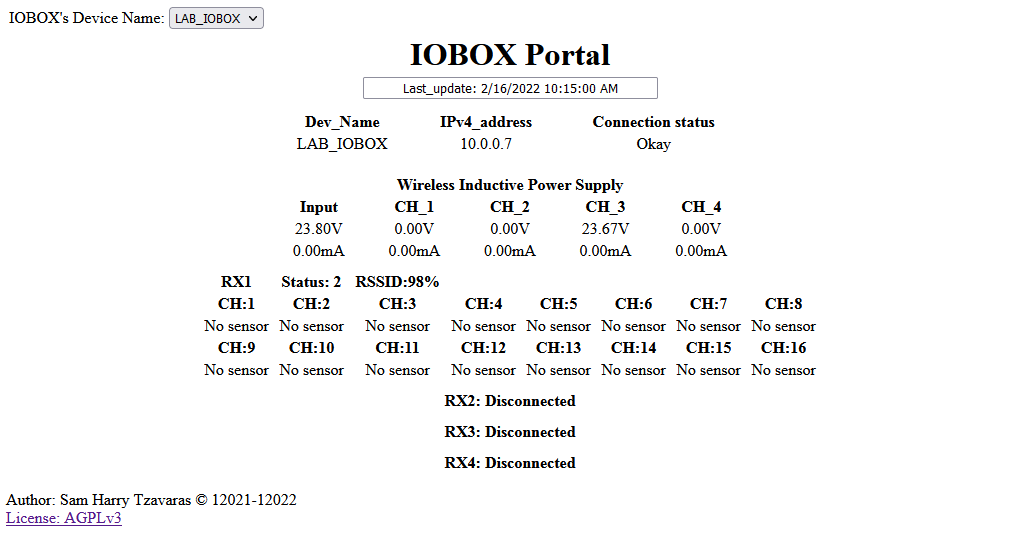
\includegraphics[width=4in,angle=0]{../art/Morfeas_web_if/Morfeas_web_IOBOX_if_UI.png}}
	\caption{Example of Morfeas WEB IOBOX-if UI}
	\label{fig:IOBOX-if_UI}
\end{figure}